\documentclass[11pt, oneside]{article}   	% use "amsart" instead of "article" for AMSLaTeX format
\usepackage{geometry}                		% See geometry.pdf to learn the layout options. There are lots.
\geometry{letterpaper}                   		% ... or a4paper or a5paper or ... 
\usepackage{graphicx}	
\usepackage{amssymb}

\title{Response Paper 2}
\author{Abhi Agarwal}
\date{}							
\begin{document}
\maketitle

\par Darwin travels from Porto Praya (Cape Verde Islands) on the coast of West Africa to Rio de Janeiro to Maldonado in the first three chapters. The first couple chapters are around change and his development in the travels. The first couple chapters paint a picture of Darwin that shows that he was curious, but in my opinion fragile. The way he got seasick shows that he's not represented as a strong man (in those days people who traveled at sea were depicted as powerful men), but depicted as young and intelligent (Well - he wasn't really depicted as he writes it, but the descriptions of how he was seasick does paint an image.). He was very different to the image I had of his family or well-read english men of the time.

\par Having done some background reading - I think it was interesting to do some analysis on the letters that Darwin, his uncle, and his dad exchanged. His dad brought up some interesting issues - one which I think summarized as the voyage being a waste of Darwin's time, and the voyage being a excuse for Darwin to move professions. I find it quite hard to believe that Darwin was able to convenience his uncle to change his father's mind about those things. It's quite interesting, and I was very curious in trying to figure out what Darwin told his uncle regarding those issues and how he convinced him. His father also pointed out the fact that other people rejected the other to go on the Voyage (the other person Fitzroy asked) and why he hadn't joined - and it would just be interesting to see Darwin's motivation beforehand.

\par Just reading the first couple chapters it was quite clear of the mental development that had happened with Darwin on the boat. It was also incredibly amusing, and quite interesting to realize that the research that they did advanced the fields of botany, zoology, and geology. It's quite easy to realize that he had a passion and appetite for exploration, discovery, and to tinker with things. He was quite observant, and he presented his findings and his thoughts very clearly. 

\par My perception Darwin changed quite a lot during the first couple chapters. At one point he was looking at these indigenous creatures, and he perceived them to being lower than household animals. This was quite shocking to me as looking from the perspective of knowing his theory it seems a little strange, but when I thought about it it's interesting as it shows his mental development. It shows how he was naive and hadn't seen the world, but this trip changed his life and gave him a new perspective of the world.

\par As mentioned in class Darwin spent three years out of five years on land as he got seasick. Most of his own observations were looking at samples, and experiencing occurrences with different cultures and tribes. Fitzroy banned Darwin from the ship when the topic of slavery came up, which I think was interesting. It shows the perception of the higher class of people (Not of Darwin) at that particular time. 

\par I've also attached a really incredible map - Incase you haven't seen it before! It's just the plotting of how he travels the world!

\par 

\par 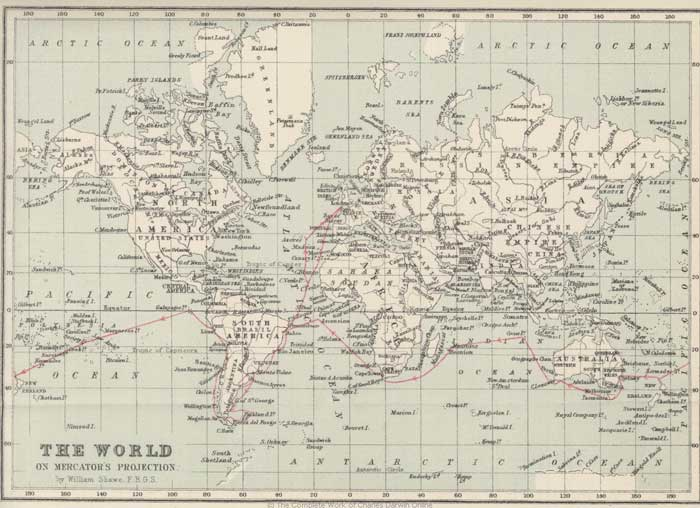
\includegraphics[scale=0.6]{map.jpg}

\end{document}